% !TeX encoding = UTF-8
% !TeX spellcheck = en_US
% !TeX root = ../main.tex

\chapter{Localization of orbit perturbations}
\label{sec:localization}

 A correction, as adapted as it can be, will never be perfect. Instead of dealing with the effects of the perturbation, its sources can first be investigated. When all possible sources are found and removed or isolated, a correction algorithm can be applied to the remaining perturbations, which will hopefully yield to better results.
 
 If no source is really obvious (e.g. a non-isolated transformer, the \SI{50}{\hertz} perturbation of the main power), the orbit itself can give some hints to localize it. One local perturbation affects indeed the whole revolution. It results in an oscillation across the orbit which, because of the closed orbit property, will brutally change its angle at the position of the source  brutally changes its angle (see \cref{fig:kick}). This position is termed \textit{kick}.

\begin{figure}[!h]
	\centering
	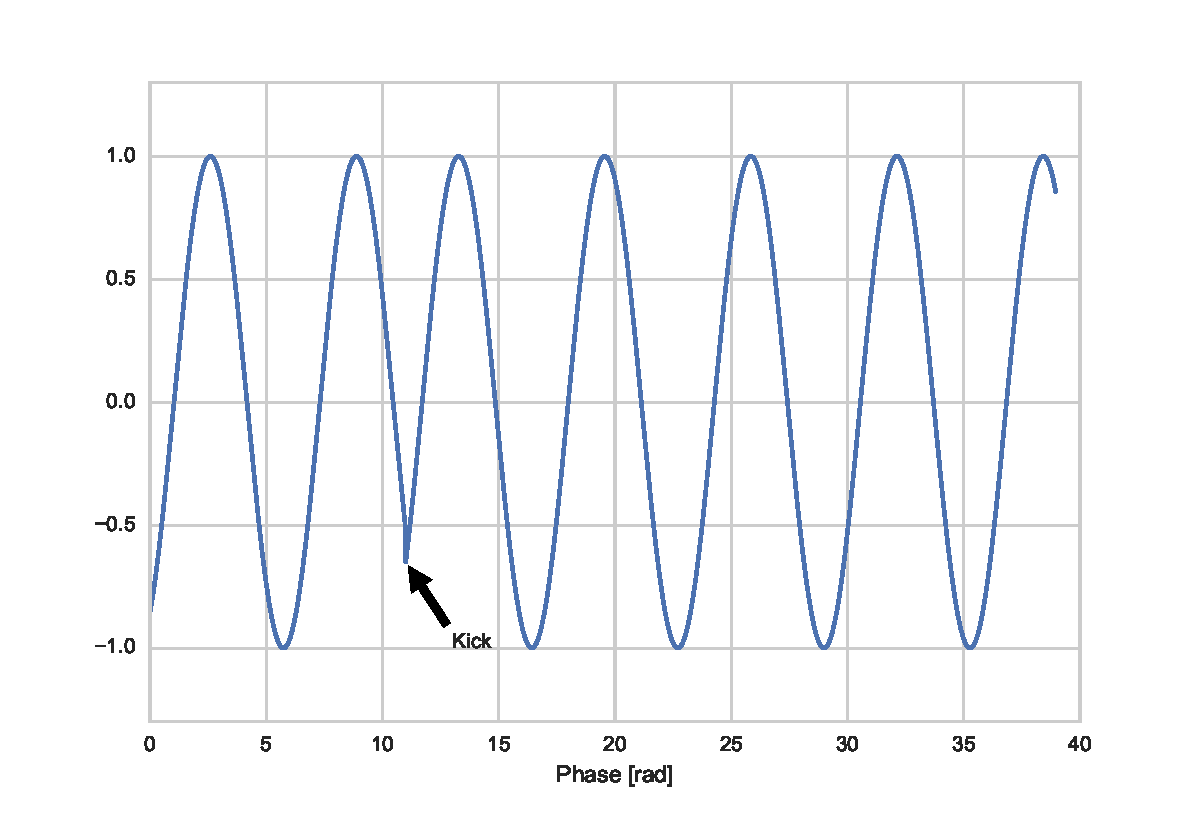
\includegraphics[width=.9\linewidth]{img/kick}
	\caption{\label{fig:kick}Example of kick in the orbit}
\end{figure}

Two types of perturbations will be described in this section:
\begin{itemize}
	\item static perturbations, which can be  for instance a malfunctioning magnet,
	\item harmonic perturbations, i.e. a perturbation at a given frequency, which can be for instance the \SI{50}{Hz} magnetic field of the main power or the \SI{10}{Hz} field due to a bad isolated power supply.
\end{itemize}

\section{Static perturbation}
\label{sec:loc_static}

\subsection{Theoretical setting of the problem}
The problem is described with the betatron phase variable 
\begin{equation}
\Psi = \int\limits_{0}^s \frac{d\sigma}{\beta(\sigma)}.
\end{equation}

The spatial variable $s$ is only used to have a connection between the result and the actual ring. The explanation will be led in the horizontal plane (with the $x$ variable), but is also valid in the vertical one ($y$).

Let one kick be at $\Psi = \hat{\Psi}$. The orbit is modified and oscillates with a constant period of \SI{2 \pi}{\radian}. Because there is \emph{only one} kick and according to the closed orbit condition, the oscillation after the kick will be stable for one revolution. Furthermore, the orbit must be continuous on all points, thus at the kick position too. This is illustrated in \cref{fig:kick}.

Two revolutions are considered, in order to be sure to find one full revolution without kick. Let $\Psi_\mathrm{ext} \in [0, 4 \pi Q]$ be this new phase (\textit{ext} for extended). The phase $\hat\Psi$ where the kick happens is the one so that 
\begin{equation}
\exists (b, c) \in \mathbb{R}^2:
\forall \Psi \in [\hat\Psi, \hat\Psi + 2 \pi Q], \quad
x(\Psi) = b \sin(\Psi + c)
\end{equation}

This problem has 3 unknowns which should be determined: $\hat\Psi, b, c$. 

\subsection{Practical setting}
In order to know the position of the orbit, BPMs are used.

Only $m$ BPMs are distributed around the orbit (in BESSY~II, $m=128$). The previous variable can thus be described in a vectorial form
\begin{align}
\begin{cases}
\vec{\Psi} = [\Psi_0, \Psi_1, ..., \Psi_{m-1}] \\
\vec{x} = [x_0, x_1, ..., x_{m-1}]
\end{cases} \quad \mathrm{and} \quad
\begin{cases}
\vec{\Psi}_\mathrm{ext} = [\vec{\Psi}, \vec{\Psi}+2\pi Q ]\\
\vec{x}_\mathrm{ext} = [\vec{x}, \vec{x}]
\end{cases}
\end{align}

\subsection{Solving the problem}

The problem is solved in two steps: first the sine that fits at best the orbit is determined, and second the position of the kick verifying the closed orbit condition (or continuity condition) is found.

An algorithm is designed to find a sine over a revolution, beginning at each BPM and keep the one that fits at best:
\begin{align}
\forall~k \in \, &[0,m-1], \nonumber \\
&\begin{cases}
\vec{\Psi}^k = [\vec{\Psi}_\mathrm{ext}(k), \vec{\Psi}_\mathrm{ext}(k+1), \cdots,  \vec{\Psi}_\mathrm{ext}(k+m-1)]\\
\vec{x}^k = [\vec{x}_\mathrm{ext}(k), \vec{x}_\mathrm{ext}(k+1), \cdots,  \vec{x}_\mathrm{ext}(k+m-1)]\\
\tilde{\vec{x}} = \mathtt{fit\_sine}(\vec{x}^k, \vec{\Psi}^k)
\end{cases}
\end{align}

It is then defined
\begin{equation}
k_0 = \underset{k \in [0, m-1]}{\textrm{argmin}}\{||\tilde{\vec{x}}-\vec{x}^k||_2\}
\end{equation}

If there where no noise in the signal, and if the number $m$ of BPMs was infinite, then the kick would be exactly at $\Psi_{k_0}$. However in the real case (with noise), it can only be said that the kick is around $\Psi_{k_0}$, and the closest sine is $\tilde{x}(\Psi) = b \sin(\Psi + c)$. 

To find the exact position of the kick, the property of closed orbit is used: the orbit must be continuous also at the kick phase, which means that $\hat{\Psi}$ is the solution of
\begin{align}
b \sin(\Psi + c) &= b\sin(\Psi+c+2 \pi Q),\\
& \mathrm{with}~ \Psi \in [\Psi_{k_0}-A, \Psi_{k_0}+A] , A>0 \nonumber
\end{align}
\begin{align}
&\begin{cases}
\Psi + c &\equiv \Psi + c + 2 \pi Q \pmod{2 \pi} \\
\Psi + c &\equiv \pi - (\Psi + c + 2 \pi Q) \pmod{2 \pi}
\end{cases} \nonumber\\
\iff &\begin{cases} 
2 \pi Q &\equiv 0\pmod \pi \qquad\qquad\textit{(Never true)}\\
\Psi &\equiv \left(\frac{1}{2} - Q\right) \pi - c \pmod \pi
\end{cases} \nonumber
\end{align}

The only possible solutions have the form
\begin{equation}
 \Psi \equiv \left(\frac{1}{2} - Q\right) \pi - c \pmod \pi.
\end{equation}
As the kick is the closest solution to $\Psi_{k_0}$, a constant $K$ is searched so that
\begin{align}
&\left(\frac{1}{2} - Q\right) \pi - c + K \pi  \leq \Psi_{k_0} \leq \left(\frac{1}{2} - Q\right) \pi - c + (K+1) \pi \\
\iff  &\left(Q - \frac{1}{2}\right) + \frac{\Psi_{k_0} + c}{\pi}\leq K \leq \left(Q - \frac{1}{2}\right) + \frac{\Psi_{k_0} + c}{\pi} +1 \\
\iff & K = \left\lfloor \left(Q - \frac{1}{2}\right) + \frac{\Psi_{k_0}+c}{\pi} \right\rfloor
\end{align}
and the two remaining possible values are
\begin{equation}
\left\lbrace \left(\frac{1}{2} - Q\right) \pi - c + K \pi , \quad \left(\frac{1}{2} - Q\right) \pi - c + (K+1) \pi\right\rbrace
\end{equation}
the kick being chosen as the closest one from $\Psi_{k_0}$.

\subsection{Finding the good sine}
Several methods are possible to find the best matching sine, for example by using:
\begin{itemize}
	\item a pseudo-inversion
	\item a scalar-product with a sine (resp. a cosine)
\end{itemize}

\paragraph{Pseudo-inversion}
The problem can be set as a linear equation problem as follow.
\begin{align}
&\forall k \in [0,m-1], \tilde{x}(\Psi_k) = a_1 \sin(\Psi_k) + a_2 \cos(\Psi_k) + a \nonumber \\
%
\implies &
\begin{pmatrix}
1 & \sin(\Psi_0) & \cos(\Psi_0) \\
1 & \sin(\Psi_1) & \cos(\Psi_1) \\
\vdots & \vdots & \vdots \\
1 & \sin(\Psi_{m-1}) & \cos(\Psi_{m-1}) \\
\end{pmatrix}
\begin{pmatrix}
a \\ a_1 \\ a_2
\end{pmatrix}
=
\begin{pmatrix}
x_0 \\ x_2 \\ \vdots \\ x_{m-1}
\end{pmatrix} \nonumber
\\
%
\implies &
\begin{pmatrix}
a \\ a_1 \\ a_2
\end{pmatrix}
= 
\mathrm{pseudo\_inv}
\begin{pmatrix}
1 & \sin(\Psi_0) & \cos(\Psi_0) \\
1 & \sin(\Psi_1) & \cos(\Psi_1) \\
\vdots & \vdots & \vdots \\
1 & \sin(\Psi_{m-1}) & \cos(\Psi_{m-1}) \\
\end{pmatrix}
\begin{pmatrix}
x_0 \\ x_2 \\ \vdots \\ x_{m-1}
\end{pmatrix}
\end{align}

The pseudo inverse is calculated in \texttt{Matlab} with 
\begin{verbatim}
        a = M\x
\end{verbatim}
and in \texttt{Python} with the least-squares method
\begin{verbatim}
        a = numpy.linalg.lstsq(M, x).
\end{verbatim}

\paragraph{Scalar product with a sine (resp. cosine)}
Since the orbit is expected to be written as
\begin{equation*}
x(\Psi) = a+ a_1 \sin(\Psi) + a_2 \cos(\Psi)
\end{equation*}
it can also be described as
\begin{equation}
x(\Psi) = \scal{x}{1} + \scal{x}{\sin} \sin(\Psi) + \scal{x}{\cos} \cos(\Psi)
\end{equation}
with $\scal{f}{g}$ being the scalar product for real functions: $\int_T f(t)g(u)dt$.

In the numerical case, the scalar product is approximated by its vectorial counterpart by
\begin{align*}
\scal{\vec{f}}{\vec{g}}: \quad
 &\mathcal{R}^n \times \mathcal{R}^n \longrightarrow \mathcal{R} \\
 & (\vec{f},\vec{g}) \quad\longmapsto \quad \frac{1}{n}\sum\limits_{k=0}^{n-1} f_i g_i
\end{align*}

\paragraph{Coefficient format}
By defining $b = \sqrt{a_1^2+a_2^2}$ and $c = \mathrm{atan2}(a_2, a_1)$ the previous formulas can be written
\begin{equation*}
\tilde{x}(\Psi) = a + a_1 \sin(\Psi) + a_2 \cos(\Psi) = a + b \sin(\Psi + c).
\end{equation*} 

\subsection{Results}

\section{Harmonic perturbations}
\todo[inline]{Linear system: perturbation f = source f}
Some perturbations can be purely harmonic. The example of the \SI{50}{\hertz} field generated by the main power is an obvious one that cannot be easily isolated. \todo{figure fft signal}

The spectrum of orbit is given in figure XXX. 

In this section, the perturbation is supposed harmonic with a given frequency $f$. 

As the perturbation has a known frequency, its complex amplitude can be extracted from the signal of each BPM with a Fourier transform:

\begin{equation}
\forall i \in [1, \mathrm{BPM\_nb}], \qquad 
\begin{cases}
\vec{X}_i = \mathrm{FFT}(\vec{x}_i) \\
c_i = \vec{X}_i(f)
\end{cases}
\end{equation}

\subsection{Case of a unique perturbation source}
If the perturbation is unique, then all complex amplitude exactly describe the same sine of frequency $f$ and phase $\alpha_0$. The complex vector $\vec{c}$ can thus be fully described with $\vec{\hat{c}}$, which is real.

\begin{align}
&\alpha_0 = \underset{\alpha \in [0, 2\pi]}{\textrm{argmin}}\{\mathcal{R}e (\vec{c} \cdot e^{-j\alpha}) \} \label{eq:harm_perturb_opt}\\
&\vec{\hat{c}} = \mathcal{I}m (\vec{c} \cdot e^{-j\alpha_0})
\end{align}

The new signal $\vec{\hat{c}}$ can be used as an orbit signal: each BPM have one orbit amplitude. The kick can be extracted from it with the previous method described in \cref{sec:loc_static}.

\remark To achieve the phase optimization given in \cref{eq:harm_perturb_opt}, the Karhunen–Loève transform (or principal component analysis) can be used~\cite{book:wang_2012}. A description of the algorithm is given in \cref{apx:KLT}. If the results are exactly the same, this allows the problem to be solved within a broader theoretical setting. The goal is not anymore to see the cosine part vanish but to deal with the perturbation space in which the distortion is the largest. In theory, dealing with each principal component would allow to find the position of each perturbation source.

\subsection{Case of several perturbation sources}
If there are several perturbation sources, a $\alpha_0$ that let the cosine part vanish cannot be found. 


\subsection{Results}

